\documentclass[11pt]{article}
\usepackage[margin=1in]{geometry}    
\usepackage{stackengine,graphicx}
\usepackage{caption}
\usepackage{subcaption}
\usepackage{indentfirst}
\usepackage{graphicx}
\usepackage{kbordermatrix}
\usepackage{physics}
\usepackage{mathtools}
\usepackage{listings}
\usepackage{float}
\usepackage{xcolor}
\usepackage{amsmath}
\definecolor{codegreen}{rgb}{0,0.6,0}
\definecolor{codegray}{rgb}{0.3,0.3,0.3}
\definecolor{codepurple}{rgb}{0.58,0,0.82}
\definecolor{backcolour}{rgb}{0.97,0.97,0.97}
\definecolor{mygreen}{RGB}{28,172,0} % color values Red, Green, Blue
\definecolor{mylilas}{RGB}{170,55,241}

\lstset{language=Matlab,%
    basicstyle=\ttfamily,
    breaklines=true,%
    morekeywords={matlab2tikz},
    keywordstyle=\color{blue},%
    morekeywords=[2]{1}, keywordstyle=[2]{\color{black}},
    identifierstyle=\color{black},%
    stringstyle=\color{mylilas},
    commentstyle=\color{mygreen},%
    showstringspaces=false,%without this there will be a symbol in the places where there is a space
    numbers=left,%
    numberstyle={\tiny \color{black}},% size of the numbers
    numbersep=9pt, % this defines how far the numbers are from the text
    emph=[1]{for,end,break},emphstyle=[1]\color{red}, %some words to emphasise
    %emph=[2]{word1,word2}, emphstyle=[2]{style},    
}

\usepackage[superscript,biblabel]{cite}
\usepackage{amsthm, amsmath, amssymb}
\DeclareMathOperator*{\argmin}{\arg\!\min}
\usepackage{setspace}\onehalfspacing
\usepackage[loose,nice]{units}  
\usepackage [english]{babel}
\usepackage{array,booktabs}
\usepackage [autostyle, english = american]{csquotes}
\MakeOuterQuote{"}
\title{Homework 3 \large \\ CAAM 28200: Dynamical Systems with Applications}
\author{Kameel Khabaz}
\date{\today}
\frenchspacing     
\begin{document}
\maketitle

\section*{Problem 2: Section 2.2}
I wrote the script below to show that my pattern of matrix exponentiation holds out to k = 10. The pattern is the following:
$$ A^k = \begin{bmatrix} (k-1)(-1)^{k-1} & k(-1)^{k-1} \\
	k(-1)^k  & (k+1)(-1)^k \end{bmatrix}$$

My code and output are below:
\begin{lstlisting}{language=Matlab}
% Problem 2  Script for matrix exponential
% Compare multiplication and with pattern
A = [0 1; 
    -1 -2];

for k = 0:10
    disp("Exponential A^" + k);
    disp(A^k)
    disp("Exponential A^" + k + " Using Pattern");
    disp(pattern(k))
end 

function [A] = pattern(k)
    A = [(-1)^(k-1) * (k-1)  k * (-1)^(k-1); 
         (-1)^k * k          (k+1) * (-1)^k];
end 
\end{lstlisting}
\begin{lstlisting}
Exponential A^0
     1     0
     0     1

Exponential A^0 Using Pattern
     1     0
     0     1

Exponential A^1
     0     1
    -1    -2

Exponential A^1 Using Pattern
     0     1
    -1    -2

Exponential A^2
    -1    -2
     2     3

Exponential A^2 Using Pattern
    -1    -2
     2     3

Exponential A^3
     2     3
    -3    -4

Exponential A^3 Using Pattern
     2     3
    -3    -4

Exponential A^4
    -3    -4
     4     5

Exponential A^4 Using Pattern
    -3    -4
     4     5

Exponential A^5
     4     5
    -5    -6

Exponential A^5 Using Pattern
     4     5
    -5    -6

Exponential A^6
    -5    -6
     6     7

Exponential A^6 Using Pattern
    -5    -6
     6     7

Exponential A^7
     6     7
    -7    -8

Exponential A^7 Using Pattern
     6     7
    -7    -8

Exponential A^8
    -7    -8
     8     9

Exponential A^8 Using Pattern
    -7    -8
     8     9

Exponential A^9
     8     9
    -9   -10

Exponential A^9 Using Pattern
     8     9
    -9   -10

Exponential A^10
    -9   -10
    10    11

Exponential A^10 Using Pattern
    -9   -10
    10    11
\end{lstlisting}

\section*{Problem 2: Section 2.3}
I now tested plotting solution trajectories for an n-term approximation for the matrix exponential. My code and plots are shown below:
\begin{lstlisting}{language=Matlab}
%% Crticially Damped Oscillator Matrix Exponential Approximation
A = [0 1; 
    -1 -2];

% Solution trajectories are given by y(t) = expo(At) * y(0)
close all
figure();
set(gcf,'Position',[0 0 800 1000])
t = linspace(0,5,100);
z0 = [1; 1];
solns = nan(2,length(t));

subplot(3,2,1);
n = 1
solve_plot(n,A,t,z0);

subplot(3,2,2);
n = 3
solve_plot(n,A,t,z0);

subplot(3,2,3);
n = 5
solve_plot(n,A,t,z0);

subplot(3,2,4);
n = 7
solve_plot(n,A,t,z0);

subplot(3,2,5);
n = 9
solve_plot(n,A,t,z0);

subplot(3,2,6);
n = 10
solve_plot(n,A,t,z0);
exportgraphics(gcf,"n_approx_trajs.eps")
function solve_plot(n,A,t,z0)
    for i = 1:length(t)
        solns(:,i) = soln_exp_approx(A,t(i),n,z0);
    end
    hold on
    di = min(find(abs(solns(1,:)) > 2))
    xline(t(di),'--r','LineWidth',1.5)
    h1= plot(t,solns(1,:),'Color','k','LineWidth',2);
    h2 = plot(t,solns(2,:),'Color','k','LineWidth',2,'LineStyle','--');
    title("$ n = " + n + " $",'Interpreter','latex')
    set(gca,'FontSize',30,'FontName','times')
    xlabel("$t$",'Interpreter','latex')
    ylabel('$z(\tau)$','Interpreter','latex')
    lgd = legend([h1 h2], "z_1","z_2")
    lgd.Location = "northwest";
    lgd.FontSize = 18;
    
end 

function [soln] = soln_exp_approx(A,t,n,z0)
    expA = [1 0; 0 1];
    for k = 1:n
        expA = expA + (1/factorial(k)) .* (A .*t )^k;
    end
    soln = expA * z0;
end 
\end{lstlisting}

In the plot in Figure \ref{fig}, I approximated the matrix exponential $\sum_{k=0}^n \frac{1}{k!}(At)^k$ for $n = 1$ to $n = 10$ and plotted trajectories starting from $z(0) = [1,1]$, which corresponds to an initial position and velocity of $1$. I then plotted the $z_1$, or position, variable as a solid line and $z_2$, or the velocity variable, as a dashed line. I then plotted the time point at which the solution diverges (chosen simply as the position exceeding twice the initial position) as a red dashed vertical line. This figure clearly shows that as $n$ increases, the red line shifts to the right, which means that the $n$-term matrix exponential approximation converges towards the true trajectory for more time. At early times, as $n$ increases, the approximate trajectory converges more towards the true trajectory (which we know from a critically damped oscillator should be a consistent decrease in both the position and velocity of the oscillator). However, for all of these approximations, regardless of $n$, the trajectory diverges at later times. This is because an exponential is a power series, and infinitely many terms are needed. Here, we are cutting off that series and including only a small number of terms, so what we get is definitely an approximation. Furthermore, each additional term of the approximation represents a higher-order behavior of the exponential function that contributes a smaller and smaller amount to the overall approximation. Thus, at early times, the function's behavior can be captured with only lower-order terms, but as one goes farther and farther from the $t=0$ point, higher order terms are needed. We can see this in Figure \ref{fig2}, in which I include $100$ terms for the approximation and obtain a much more accurate solution trajectory up to $t = 10$. However, even here, we see that if we increase the time enough, as in the right figure, the approximation will eventually diverge.

\begin{figure}[h]

\includegraphics[width=15cm]{n_approx_trajs.eps}
\caption{$n$-term Approximation Solution Trajectories from $z(0) = [1, 1]$}
\label{fig}
\end{figure}

\begin{figure}[h]
\centering
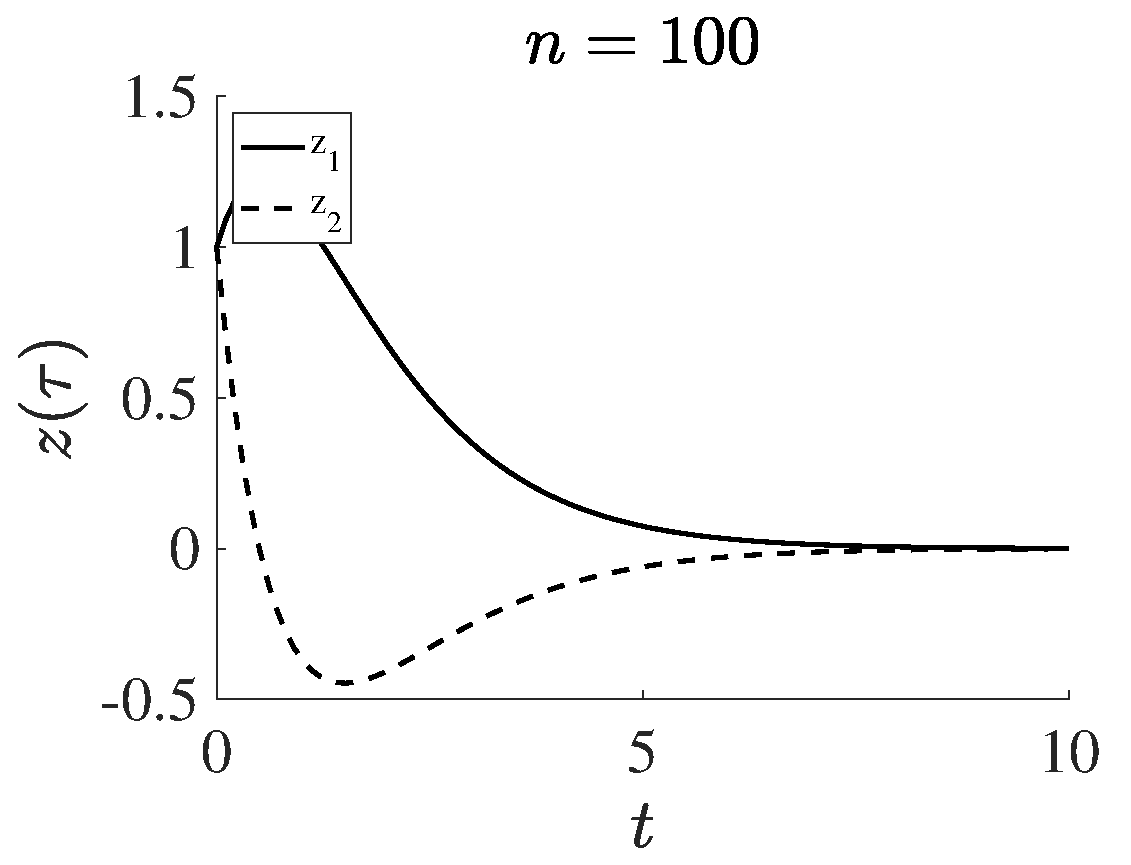
\includegraphics[width=8cm]{Approx_traj_100_term.eps}
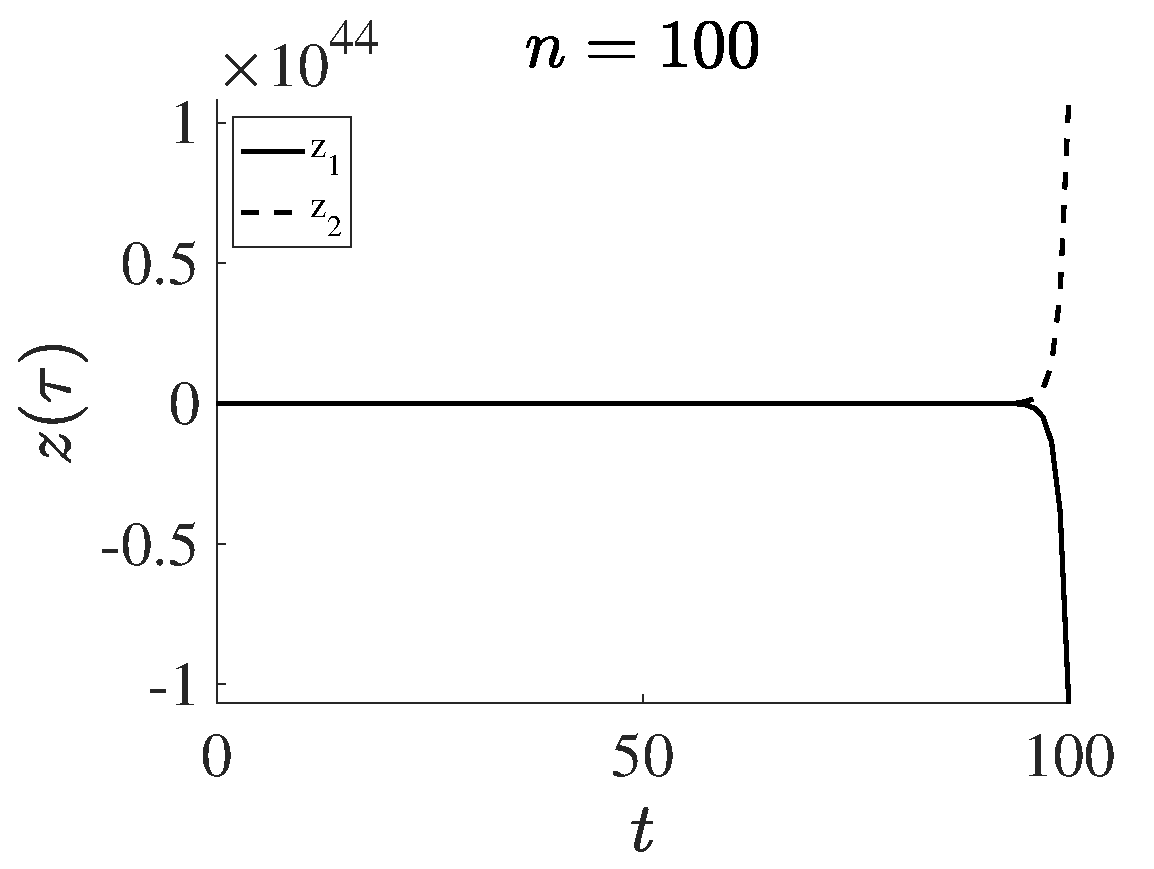
\includegraphics[width=8cm]{Approx_traj_100_term2.eps}
\caption{$100$-term Approximation Solution Trajectories}
\label{fig2}
\end{figure}
\clearpage 

\section*{Problem 2: Section 2.7}
Below, I show my code and plots using the explicit form of the matrix exponential (defined in number 5) to plot the exact solution starting from $z(0) = [1,1]$.

\begin{lstlisting}{language=Matlab}
%% Problem 2.7 - Solution with Explicit Form of Matrix Exponential
figure()
t = linspace(0,10,100);
explicit_soln_plot(A,t,z0)
exportgraphics(gcf,"explicit_form_soln.eps")

t = linspace(0,100,100);
explicit_soln_plot(A,t,z0)
exportgraphics(gcf,"explicit_form_soln_lt.eps")
function explicit_soln_plot(A,t,z0)
    solns = nan(2,length(t))
    for i = 1:length(t)
        solns(:,i) = exp(-t(i)) * ([1 0; 0 1] + t(i) * [1 1; -1 -1]) * z0;
    end 
    hold on
    di = min(find(abs(solns(1,:)) > 2))
    if isinteger(di)
        xline(t(di),'--r','LineWidth',1.5)
    end 
    h1= plot(t,solns(1,:),'Color','k','LineWidth',2);
    h2 = plot(t,solns(2,:),'Color','k','LineWidth',2,'LineStyle','--');
    title("Explicit Form of Matrix Exponential",'Interpreter','latex')
    set(gca,'FontSize',30,'FontName','times')
    xlabel("$t$",'Interpreter','latex')
    ylabel('$z(\tau)$','Interpreter','latex')
    lgd = legend([h1 h2], "z_1","z_2")
    lgd.Location = "northeast";
    lgd.FontSize = 18;
    
end 
\end{lstlisting}
 When comparing Figure \ref{fig2} to Figure \ref{exact}, we see that using the explicit form for the matrix exponential results in a solution trajectory that matches the expected trajectory even at long time spans. While using an partial expansion of the matrix exponential means that the excluded higher-order terms result in a solution diverging at large time scales, using the exact form of the exponential includes all higher-order terms and thus results in the correct trajectory. Note how both the approximate solutions (with large $n$) and the exact solution result in similar behavior at small time spans (such as up to $t = 10$ for $n = 100$).
 
 \begin{figure}[h]
 \centering
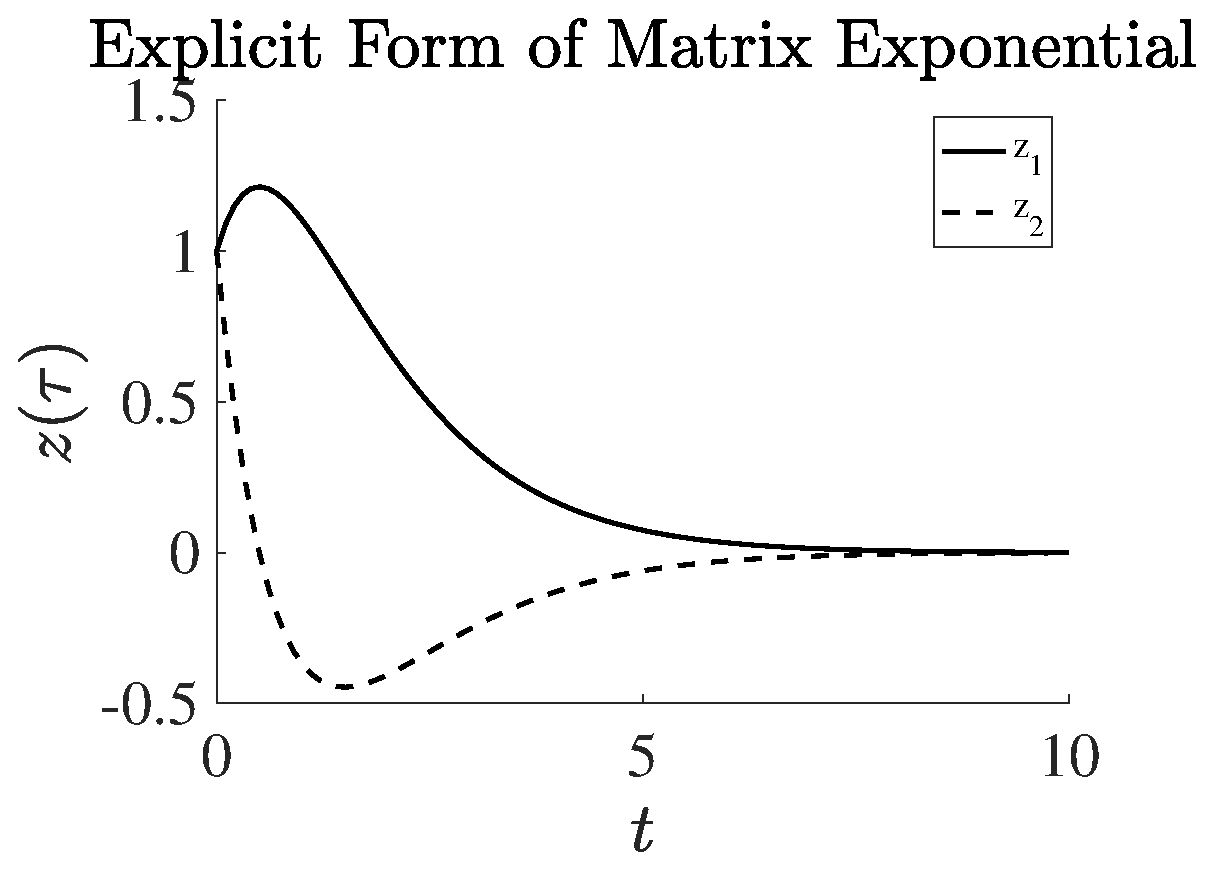
\includegraphics[width=8cm]{explicit_form_soln.eps}
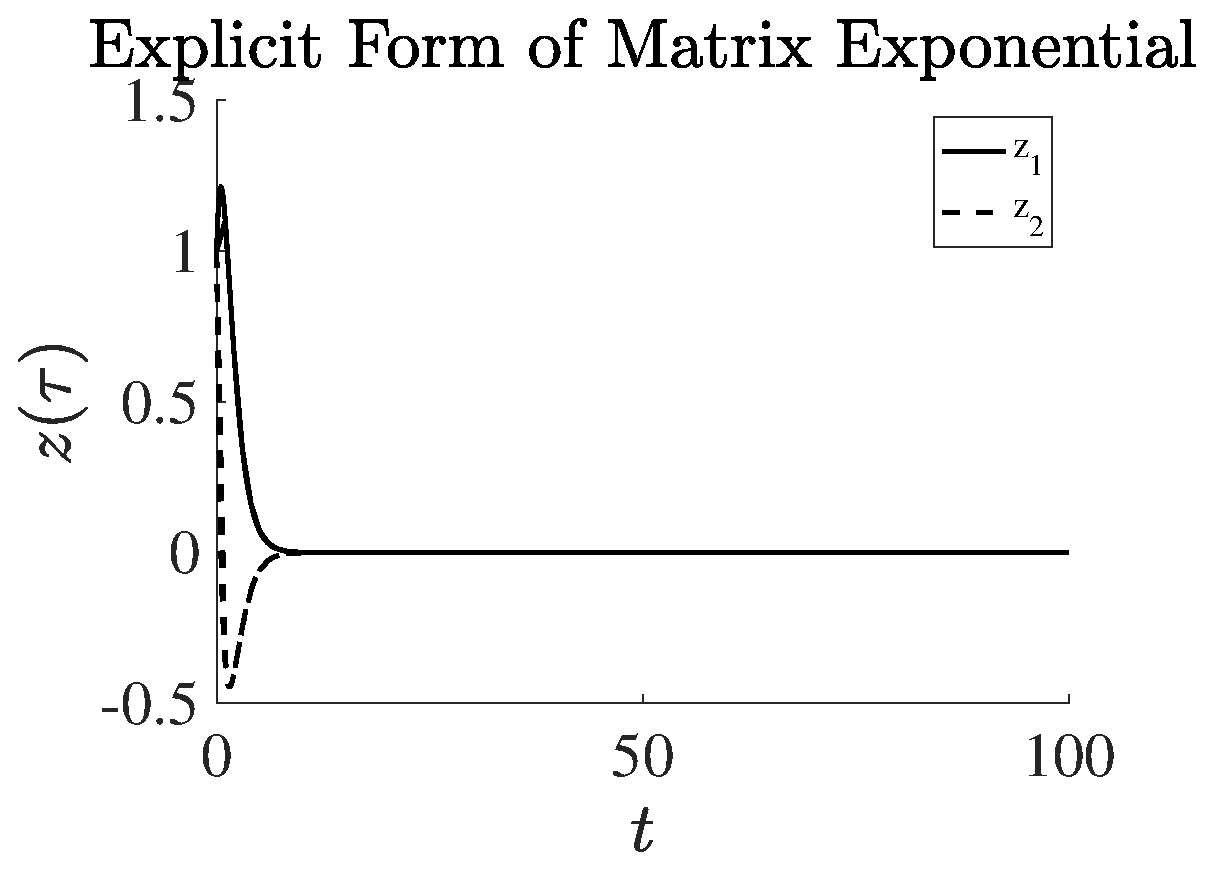
\includegraphics[width=8cm]{explicit_form_soln_lt.eps}
\caption{Exact Solution Trajectories}
\label{exact}
\end{figure}
\clearpage 

\end{document}
